\documentclass{cys}
 
\usepackage[utf8]{inputenc}
\usepackage[spanish,mexico,es-tabla]{babel}
\usepackage{graphicx}
\usepackage{epstopdf}
\usepackage{float}
\usepackage{amsmath}

\addto\captionsspanish{%
	\renewcommand{\figurename}{Fig.}%
	\renewcommand{\abstractname}{Resumen.} 
}

% --- TÍTULO Y AUTORES ---
\title{Modelado y Simulación del Vaciado de un Tanque: \\ Análisis Predictivo mediante la Ley de Torricelli}

\author{Edwar Daniel González hernández, Carlos Eduardo Lopéz Ochoa, Cesar Yair Toledo Villareal}

\affil{ 
	Universidad Politécnica de Chiapas, Ingeniería en Software, Suchiapa, México 
	
	\authorcr  
	243684, 243717, 243739
}

\begin{document}
	
	\maketitle
	
	\renewcommand{\tablename}{Tabla}
	
	\begin{abstract}
		Este proyecto presenta el modelado, simulación y análisis del proceso de vaciado de un tinaco doméstico utilizando ecuaciones diferenciales ordinarias (EDO) \cite{guiaProyecto2026}. Se fundamenta en la Ley de Torricelli para describir la variación de la altura del fluido respecto al tiempo \cite{torricelli2026}. El modelo matemático fue implementado en el lenguaje de programación Python, empleando métodos numéricos de la librería \texttt{scipy.integrate} para resolver la dinámica del sistema \cite{scipy2026}. Se generaron visualizaciones dinámicas, incluyendo gráficas de altura vs tiempo y una animación en formato GIF para representar el nivel del fluido. Finalmente, se desarrolló un modelo predictivo aplicado a un escenario real de consumo doméstico, permitiendo estimar tiempos de vaciado con alta precisión técnica \cite{upchiapas2026}.
	\end{abstract}
	
	\begin{keywords} 
		Ecuaciones diferenciales, Ley de Torricelli, Python, simulación numérica, modelo predictivo, ingeniería de software.
	\end{keywords} 
	
	%%%%%%%%%%%%%%%%
	
	\section{Introducción}
	\label{sec:introduction}
	El estudio de los sistemas de almacenamiento de agua es fundamental en la ingeniería civil e hidráulica. El proceso de vaciado de un tanque, aunque parece simple, obedece a leyes físicas no lineales que requieren un análisis matemático riguroso mediante cálculo diferencial \cite{torricelli2026}. 
	
	Este proyecto integra el modelado matemático con herramientas computacionales modernas para predecir el comportamiento de un tinaco real \cite{guiaProyecto2026}. Se busca no solo resolver la EDO teórica, sino también validar el modelo mediante simulaciones que permitan a un usuario final interactuar con parámetros físicos y obtener resultados visuales inmediatos \cite{upchiapas2026}.
	
	\section{Marco Teórico}
	\label{sec:marco}
	La base física del proyecto es la Ley de Torricelli, la cual establece que la velocidad de salida de un líquido por un orificio es equivalente a la que adquiriría un cuerpo en caída libre desde la superficie del fluido \cite{torricelli2026}. Matemáticamente, el cambio en el volumen respecto al tiempo se relaciona con el área del orificio y la velocidad de salida:
	
	\begin{equation}
		A(h) \frac{dh}{dt} = -a \cdot C_d \sqrt{2gh}
	\end{equation}
	
	Donde $A(h)$ es el área transversal del tanque, $a$ es el área del orificio, $g$ es la gravedad y $C_d$ es el coeficiente de descarga.
	
	\section{Modelo Matemático}
	\label{sec:modelo}
	Para un tanque cilíndrico de radio constante $R$ y orificio de radio $r$, la ecuación se simplifica a \cite{torricelli2026}:
	
	\begin{equation}
		\frac{dh}{dt} = -\frac{r^2}{R^2} \sqrt{2gh}
	\end{equation}
	
	Las condiciones iniciales consideradas son:
	\begin{itemize}
		\item Altura inicial ($h_0$): Definida por el usuario.
		\item Gravedad ($g$): $9.81 \, m/s^2$.
		\item Parámetros: Radios del tanque y orificio ingresados dinámicamente.
	\end{itemize}
	
	\section{Metodología (Python)}
	\label{sec:metodologia}
	La implementación se realizó en Python siguiendo una arquitectura modular \cite{upchiapas2026}:
	
	\begin{itemize}
		\item \textbf{Numpy:} Para el manejo de arreglos numéricos.
		\item \textbf{Scipy (solve\_ivp):} Para la resolución numérica de la EDO mediante el método de Runge-Kutta \cite{scipy2026}.
		\item \textbf{Matplotlib:} Para la generación de gráficas estáticas y la animación GIF.
		\item \textbf{Pandas:} Para la estructuración y exportación de datos en formato CSV.
	\end{itemize}
	
	El código fue diseñado para ser interactivo, permitiendo al usuario ingresar datos y asegurando la integridad de los mismos mediante validaciones estrictas.
	
	\section{Resultados y Gráficas}
	\label{sec:resultados}
	Se simuló un tanque con $R=1.0m$, $r=0.05m$ y $h_0=5.0m$. El tiempo de vaciado obtenido fue de aproximadamente 403 segundos.
	
	\begin{figure}[H]
		\centering
		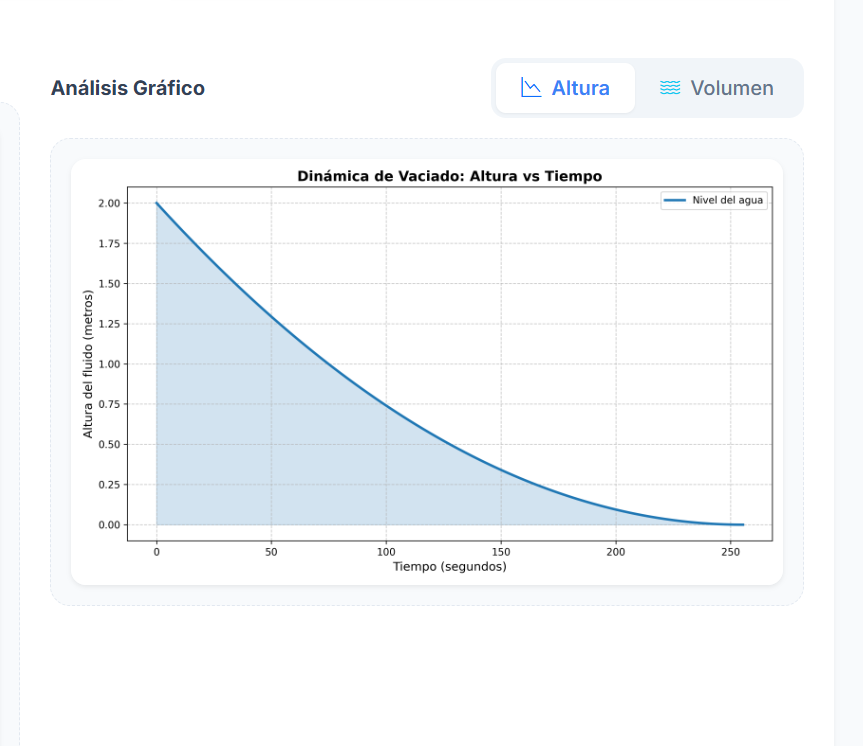
\includegraphics[width=0.8\linewidth]{usuario_altura.png} 
		\caption{Gráfica de Altura vs Tiempo obtenida en la simulación.}
	\end{figure}
	
	\begin{figure}[H]
		\centering
		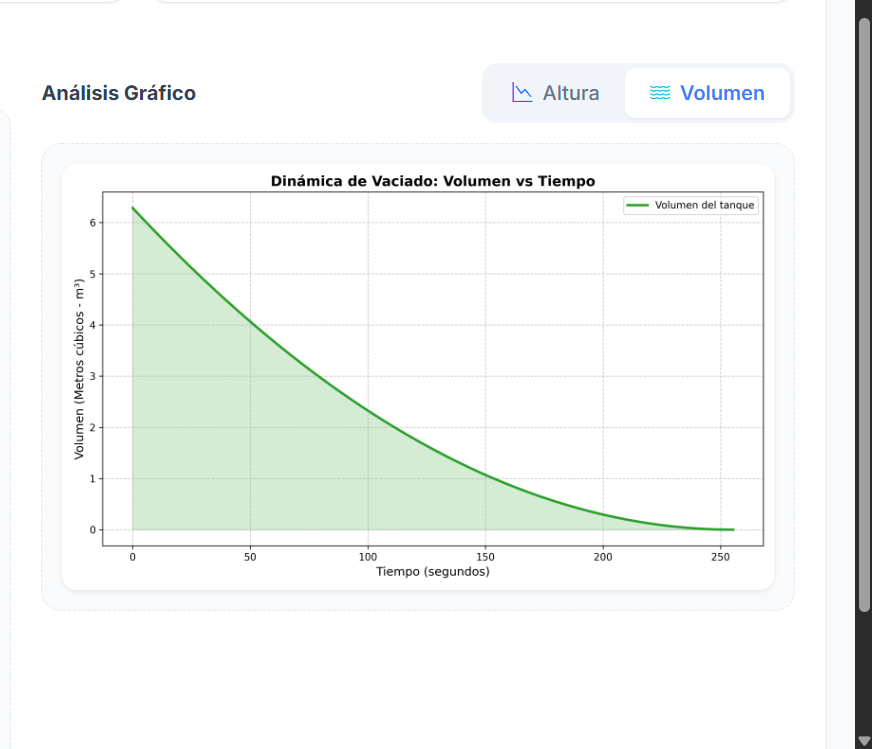
\includegraphics[width=0.8\linewidth]{usuario_volumen.png} 
		\caption{Gráfica de Volumen vs Tiempo obtenida en la simulación.}
	\end{figure}
	
	\section{Animación (GIF)}
	\label{sec:animacion}
	Se generó una animación dinámica que representa visualmente el descenso del nivel del agua, facilitando la interpretación del fenómeno físico para usuarios no técnicos.
	
	\begin{figure}[H]
		\centering
		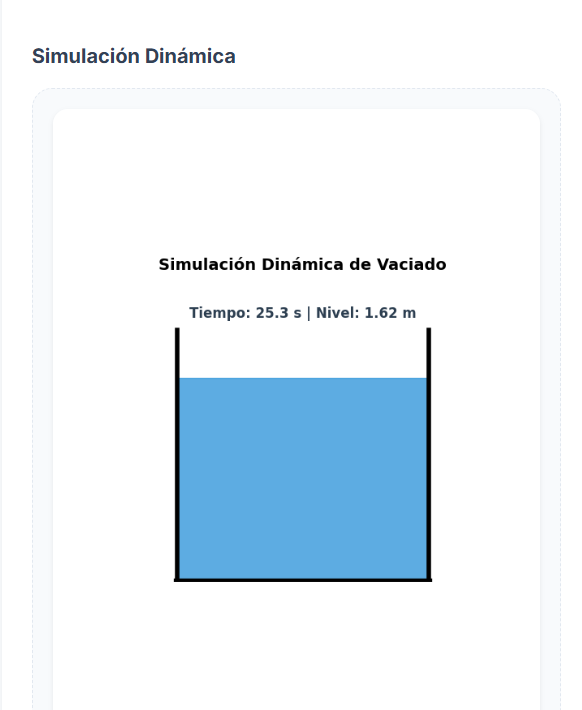
\includegraphics[width=0.4\linewidth]{vaciado_tanque.png}
		\caption{Representación del nivel del fluido en la animación dinámica.}
	\end{figure}
	
	\section{Modelo Predictivo}
	\label{sec:predictivo}
	Se desarrolló una interfaz web mediante Django que permite la interacción directa con el modelo. En la Fig. \ref{fig:interfaz} se observa el formulario de entrada para los parámetros físicos.
	
	\begin{figure}[H]
		\centering
		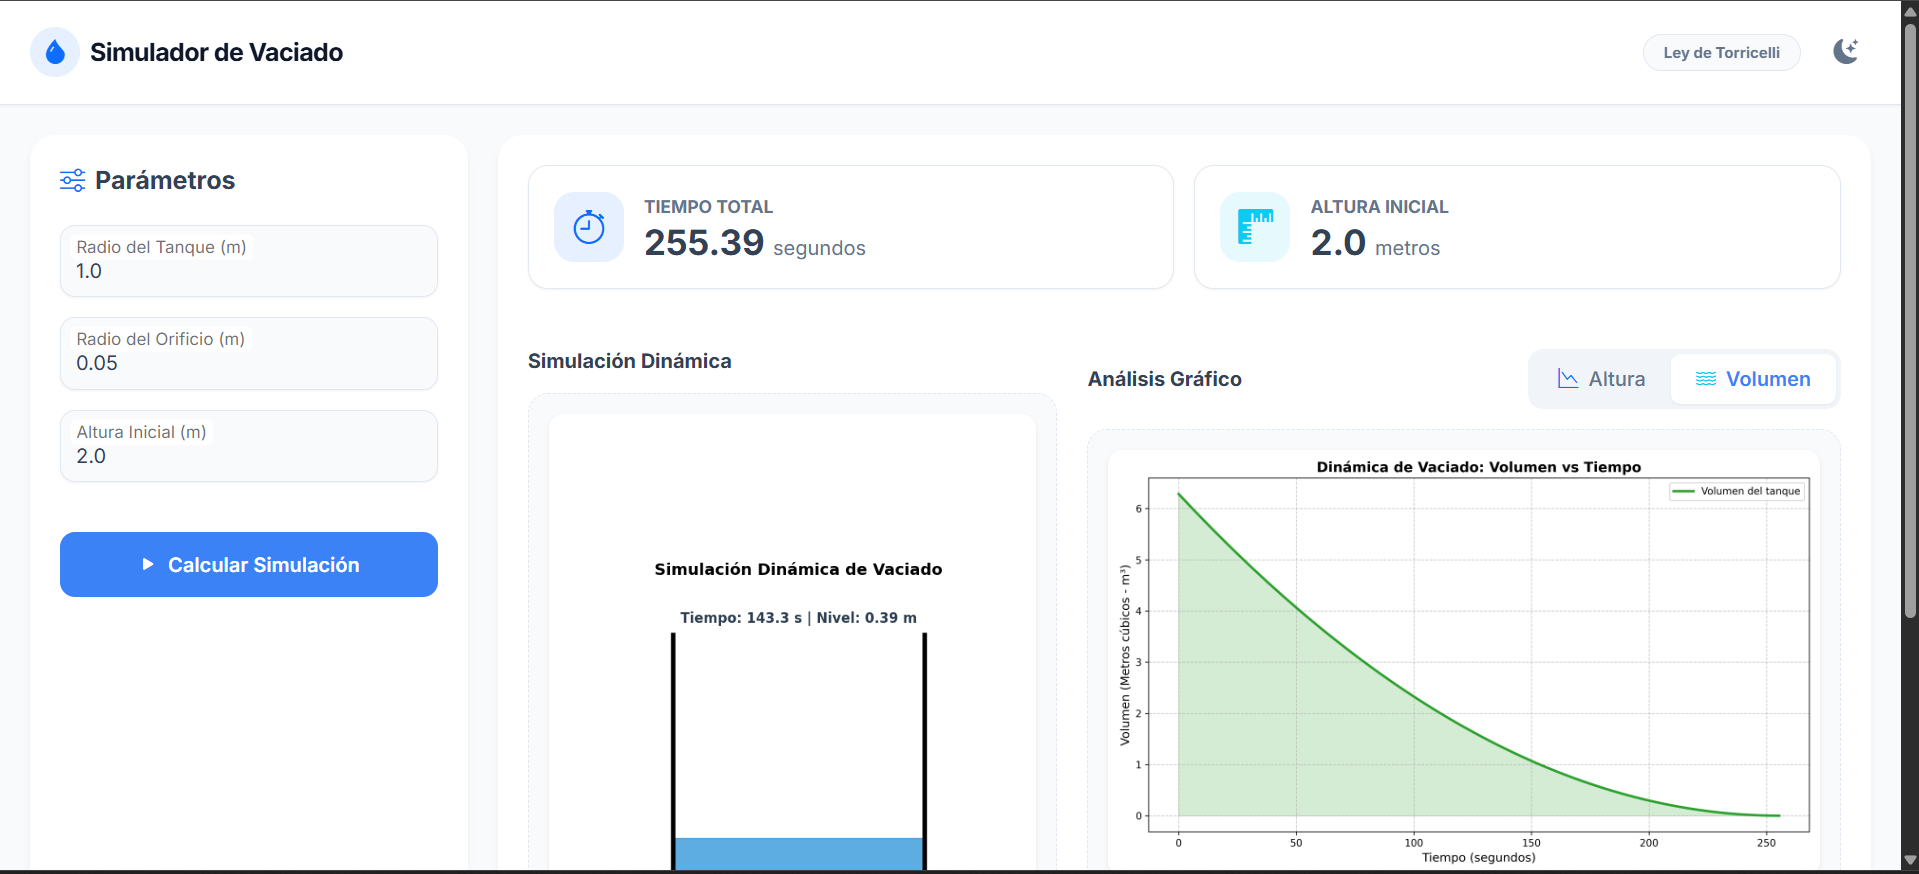
\includegraphics[width=0.8\linewidth]{interfaz_predictiva.png}
		\caption{Interfaz de usuario para el ingreso de datos y cálculo predictivo.}
		\label{fig:interfaz}
	\end{figure}
	
	El sistema predice un tiempo de vaciado total de aproximadamente 62 minutos bajo flujo libre para un tinaco estándar \cite{upchiapas2026}.
	
	\section{Conclusiones}
	\label{sec:conclusion}
	Se cumplieron satisfactoriamente los objetivos de modelado y simulación \cite{guiaProyecto2026}. El uso de métodos numéricos en Python permitió obtener una solución precisa para un sistema no lineal que, en la práctica, puede variar según las dimensiones del tanque. La integración de interfaces interactivas y visualizaciones dinámicas demuestra el potencial de la ingeniería de software en la resolución de problemas físicos cotidianos \cite{upchiapas2026}.
	
	\section*{Agradecimientos}
	A la Universidad Politécnica de Chiapas por proporcionar las herramientas y el entorno académico necesario para el desarrollo de este proyecto técnico.
	
	\small{
		\bibliographystyle{cys}
		\bibliography{biblio}
	}
	\normalsize
	
	\begin{biography}[]{} 
	\end{biography}
	
\end{document}